% Created by tikzDevice version 0.12.3.1 on 2021-04-14 10:42:54
% !TEX encoding = UTF-8 Unicode
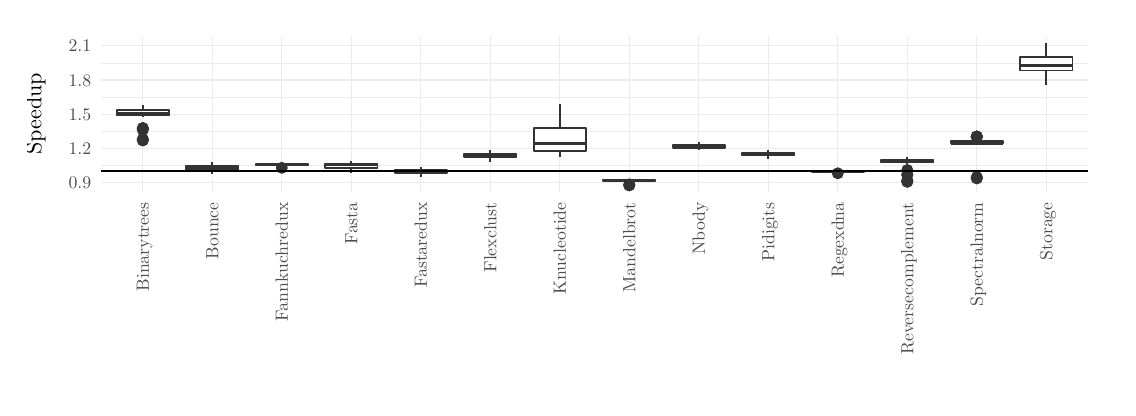
\begin{tikzpicture}[x=1pt,y=1pt]
\definecolor{fillColor}{RGB}{255,255,255}
\path[use as bounding box,fill=fillColor,fill opacity=0.00] (0,0) rectangle (390.26,130.09);
\begin{scope}
\path[clip] ( 26.53, 70.57) rectangle (383.14,127.24);
\definecolor{drawColor}{gray}{0.92}

\path[draw=drawColor,line width= 0.2pt,line join=round] ( 26.53, 80.24) --
	(383.14, 80.24);

\path[draw=drawColor,line width= 0.2pt,line join=round] ( 26.53, 92.62) --
	(383.14, 92.62);

\path[draw=drawColor,line width= 0.2pt,line join=round] ( 26.53,105.00) --
	(383.14,105.00);

\path[draw=drawColor,line width= 0.2pt,line join=round] ( 26.53,117.38) --
	(383.14,117.38);

\path[draw=drawColor,line width= 0.4pt,line join=round] ( 26.53, 74.05) --
	(383.14, 74.05);

\path[draw=drawColor,line width= 0.4pt,line join=round] ( 26.53, 86.43) --
	(383.14, 86.43);

\path[draw=drawColor,line width= 0.4pt,line join=round] ( 26.53, 98.81) --
	(383.14, 98.81);

\path[draw=drawColor,line width= 0.4pt,line join=round] ( 26.53,111.19) --
	(383.14,111.19);

\path[draw=drawColor,line width= 0.4pt,line join=round] ( 26.53,123.57) --
	(383.14,123.57);

\path[draw=drawColor,line width= 0.4pt,line join=round] ( 41.60, 70.57) --
	( 41.60,127.24);

\path[draw=drawColor,line width= 0.4pt,line join=round] ( 66.71, 70.57) --
	( 66.71,127.24);

\path[draw=drawColor,line width= 0.4pt,line join=round] ( 91.83, 70.57) --
	( 91.83,127.24);

\path[draw=drawColor,line width= 0.4pt,line join=round] (116.94, 70.57) --
	(116.94,127.24);

\path[draw=drawColor,line width= 0.4pt,line join=round] (142.05, 70.57) --
	(142.05,127.24);

\path[draw=drawColor,line width= 0.4pt,line join=round] (167.17, 70.57) --
	(167.17,127.24);

\path[draw=drawColor,line width= 0.4pt,line join=round] (192.28, 70.57) --
	(192.28,127.24);

\path[draw=drawColor,line width= 0.4pt,line join=round] (217.39, 70.57) --
	(217.39,127.24);

\path[draw=drawColor,line width= 0.4pt,line join=round] (242.51, 70.57) --
	(242.51,127.24);

\path[draw=drawColor,line width= 0.4pt,line join=round] (267.62, 70.57) --
	(267.62,127.24);

\path[draw=drawColor,line width= 0.4pt,line join=round] (292.74, 70.57) --
	(292.74,127.24);

\path[draw=drawColor,line width= 0.4pt,line join=round] (317.85, 70.57) --
	(317.85,127.24);

\path[draw=drawColor,line width= 0.4pt,line join=round] (342.96, 70.57) --
	(342.96,127.24);

\path[draw=drawColor,line width= 0.4pt,line join=round] (368.08, 70.57) --
	(368.08,127.24);
\definecolor{drawColor}{gray}{0.20}
\definecolor{fillColor}{gray}{0.20}

\path[draw=drawColor,line width= 0.4pt,line join=round,line cap=round,fill=fillColor] ( 41.60, 93.85) circle (  1.96);

\path[draw=drawColor,line width= 0.4pt,line join=round,line cap=round,fill=fillColor] ( 41.60, 93.70) circle (  1.96);

\path[draw=drawColor,line width= 0.4pt,line join=round,line cap=round,fill=fillColor] ( 41.60, 93.42) circle (  1.96);

\path[draw=drawColor,line width= 0.4pt,line join=round,line cap=round,fill=fillColor] ( 41.60, 93.13) circle (  1.96);

\path[draw=drawColor,line width= 0.4pt,line join=round,line cap=round,fill=fillColor] ( 41.60, 89.83) circle (  1.96);

\path[draw=drawColor,line width= 0.4pt,line join=round,line cap=round,fill=fillColor] ( 41.60, 89.63) circle (  1.96);

\path[draw=drawColor,line width= 0.4pt,line join=round,line cap=round,fill=fillColor] ( 41.60, 89.57) circle (  1.96);

\path[draw=drawColor,line width= 0.4pt,line join=round,line cap=round,fill=fillColor] ( 41.60, 89.32) circle (  1.96);

\path[draw=drawColor,line width= 0.6pt,line join=round] ( 41.60,100.35) -- ( 41.60,102.14);

\path[draw=drawColor,line width= 0.6pt,line join=round] ( 41.60, 98.39) -- ( 41.60, 97.69);
\definecolor{fillColor}{RGB}{255,255,255}

\path[draw=drawColor,line width= 0.6pt,line join=round,line cap=round,fill=fillColor] ( 32.18,100.35) --
	( 32.18, 98.39) --
	( 51.02, 98.39) --
	( 51.02,100.35) --
	( 32.18,100.35) --
	cycle;

\path[draw=drawColor,line width= 1.1pt,line join=round] ( 32.18, 99.16) -- ( 51.02, 99.16);

\path[draw=drawColor,line width= 0.6pt,line join=round] ( 66.71, 80.19) -- ( 66.71, 81.55);

\path[draw=drawColor,line width= 0.6pt,line join=round] ( 66.71, 78.72) -- ( 66.71, 77.10);

\path[draw=drawColor,line width= 0.6pt,line join=round,line cap=round,fill=fillColor] ( 57.30, 80.19) --
	( 57.30, 78.72) --
	( 76.13, 78.72) --
	( 76.13, 80.19) --
	( 57.30, 80.19) --
	cycle;

\path[draw=drawColor,line width= 1.1pt,line join=round] ( 57.30, 79.32) -- ( 76.13, 79.32);
\definecolor{fillColor}{gray}{0.20}

\path[draw=drawColor,line width= 0.4pt,line join=round,line cap=round,fill=fillColor] ( 91.83, 79.44) circle (  1.96);

\path[draw=drawColor,line width= 0.6pt,line join=round] ( 91.83, 80.85) -- ( 91.83, 80.97);

\path[draw=drawColor,line width= 0.6pt,line join=round] ( 91.83, 80.31) -- ( 91.83, 79.61);
\definecolor{fillColor}{RGB}{255,255,255}

\path[draw=drawColor,line width= 0.6pt,line join=round,line cap=round,fill=fillColor] ( 82.41, 80.85) --
	( 82.41, 80.31) --
	(101.24, 80.31) --
	(101.24, 80.85) --
	( 82.41, 80.85) --
	cycle;

\path[draw=drawColor,line width= 1.1pt,line join=round] ( 82.41, 80.50) -- (101.24, 80.50);

\path[draw=drawColor,line width= 0.6pt,line join=round] (116.94, 81.04) -- (116.94, 81.80);

\path[draw=drawColor,line width= 0.6pt,line join=round] (116.94, 79.33) -- (116.94, 77.55);

\path[draw=drawColor,line width= 0.6pt,line join=round,line cap=round,fill=fillColor] (107.52, 81.04) --
	(107.52, 79.33) --
	(126.36, 79.33) --
	(126.36, 81.04) --
	(107.52, 81.04) --
	cycle;

\path[draw=drawColor,line width= 1.1pt,line join=round] (107.52, 80.81) -- (126.36, 80.81);

\path[draw=drawColor,line width= 0.6pt,line join=round] (142.05, 78.55) -- (142.05, 79.68);

\path[draw=drawColor,line width= 0.6pt,line join=round] (142.05, 77.48) -- (142.05, 76.09);

\path[draw=drawColor,line width= 0.6pt,line join=round,line cap=round,fill=fillColor] (132.64, 78.55) --
	(132.64, 77.48) --
	(151.47, 77.48) --
	(151.47, 78.55) --
	(132.64, 78.55) --
	cycle;

\path[draw=drawColor,line width= 1.1pt,line join=round] (132.64, 78.09) -- (151.47, 78.09);

\path[draw=drawColor,line width= 0.6pt,line join=round] (167.17, 84.47) -- (167.17, 85.77);

\path[draw=drawColor,line width= 0.6pt,line join=round] (167.17, 83.33) -- (167.17, 81.72);

\path[draw=drawColor,line width= 0.6pt,line join=round,line cap=round,fill=fillColor] (157.75, 84.47) --
	(157.75, 83.33) --
	(176.59, 83.33) --
	(176.59, 84.47) --
	(157.75, 84.47) --
	cycle;

\path[draw=drawColor,line width= 1.1pt,line join=round] (157.75, 83.74) -- (176.59, 83.74);

\path[draw=drawColor,line width= 0.6pt,line join=round] (192.28, 93.95) -- (192.28,102.37);

\path[draw=drawColor,line width= 0.6pt,line join=round] (192.28, 85.44) -- (192.28, 83.22);

\path[draw=drawColor,line width= 0.6pt,line join=round,line cap=round,fill=fillColor] (182.86, 93.95) --
	(182.86, 85.44) --
	(201.70, 85.44) --
	(201.70, 93.95) --
	(182.86, 93.95) --
	cycle;

\path[draw=drawColor,line width= 1.1pt,line join=round] (182.86, 88.20) -- (201.70, 88.20);
\definecolor{fillColor}{gray}{0.20}

\path[draw=drawColor,line width= 0.4pt,line join=round,line cap=round,fill=fillColor] (217.39, 73.46) circle (  1.96);

\path[draw=drawColor,line width= 0.4pt,line join=round,line cap=round,fill=fillColor] (217.39, 73.18) circle (  1.96);

\path[draw=drawColor,line width= 0.4pt,line join=round,line cap=round,fill=fillColor] (217.39, 73.16) circle (  1.96);

\path[draw=drawColor,line width= 0.4pt,line join=round,line cap=round,fill=fillColor] (217.39, 73.15) circle (  1.96);

\path[draw=drawColor,line width= 0.6pt,line join=round] (217.39, 74.99) -- (217.39, 75.22);

\path[draw=drawColor,line width= 0.6pt,line join=round] (217.39, 74.68) -- (217.39, 74.38);
\definecolor{fillColor}{RGB}{255,255,255}

\path[draw=drawColor,line width= 0.6pt,line join=round,line cap=round,fill=fillColor] (207.98, 74.99) --
	(207.98, 74.68) --
	(226.81, 74.68) --
	(226.81, 74.99) --
	(207.98, 74.99) --
	cycle;

\path[draw=drawColor,line width= 1.1pt,line join=round] (207.98, 74.90) -- (226.81, 74.90);

\path[draw=drawColor,line width= 0.6pt,line join=round] (242.51, 87.76) -- (242.51, 88.67);

\path[draw=drawColor,line width= 0.6pt,line join=round] (242.51, 86.71) -- (242.51, 85.90);

\path[draw=drawColor,line width= 0.6pt,line join=round,line cap=round,fill=fillColor] (233.09, 87.76) --
	(233.09, 86.71) --
	(251.93, 86.71) --
	(251.93, 87.76) --
	(233.09, 87.76) --
	cycle;

\path[draw=drawColor,line width= 1.1pt,line join=round] (233.09, 86.93) -- (251.93, 86.93);

\path[draw=drawColor,line width= 0.6pt,line join=round] (267.62, 84.86) -- (267.62, 86.04);

\path[draw=drawColor,line width= 0.6pt,line join=round] (267.62, 83.94) -- (267.62, 82.74);

\path[draw=drawColor,line width= 0.6pt,line join=round,line cap=round,fill=fillColor] (258.20, 84.86) --
	(258.20, 83.94) --
	(277.04, 83.94) --
	(277.04, 84.86) --
	(258.20, 84.86) --
	cycle;

\path[draw=drawColor,line width= 1.1pt,line join=round] (258.20, 84.39) -- (277.04, 84.39);
\definecolor{fillColor}{gray}{0.20}

\path[draw=drawColor,line width= 0.4pt,line join=round,line cap=round,fill=fillColor] (292.74, 77.47) circle (  1.96);

\path[draw=drawColor,line width= 0.6pt,line join=round] (292.74, 78.34) -- (292.74, 78.45);

\path[draw=drawColor,line width= 0.6pt,line join=round] (292.74, 78.04) -- (292.74, 77.67);
\definecolor{fillColor}{RGB}{255,255,255}

\path[draw=drawColor,line width= 0.6pt,line join=round,line cap=round,fill=fillColor] (283.32, 78.34) --
	(283.32, 78.04) --
	(302.15, 78.04) --
	(302.15, 78.34) --
	(283.32, 78.34) --
	cycle;

\path[draw=drawColor,line width= 1.1pt,line join=round] (283.32, 78.27) -- (302.15, 78.27);
\definecolor{fillColor}{gray}{0.20}

\path[draw=drawColor,line width= 0.4pt,line join=round,line cap=round,fill=fillColor] (317.85, 78.65) circle (  1.96);

\path[draw=drawColor,line width= 0.4pt,line join=round,line cap=round,fill=fillColor] (317.85, 77.01) circle (  1.96);

\path[draw=drawColor,line width= 0.4pt,line join=round,line cap=round,fill=fillColor] (317.85, 76.89) circle (  1.96);

\path[draw=drawColor,line width= 0.4pt,line join=round,line cap=round,fill=fillColor] (317.85, 74.87) circle (  1.96);

\path[draw=drawColor,line width= 0.4pt,line join=round,line cap=round,fill=fillColor] (317.85, 74.80) circle (  1.96);

\path[draw=drawColor,line width= 0.4pt,line join=round,line cap=round,fill=fillColor] (317.85, 74.47) circle (  1.96);

\path[draw=drawColor,line width= 0.4pt,line join=round,line cap=round,fill=fillColor] (317.85, 74.40) circle (  1.96);

\path[draw=drawColor,line width= 0.6pt,line join=round] (317.85, 82.32) -- (317.85, 83.46);

\path[draw=drawColor,line width= 0.6pt,line join=round] (317.85, 81.41) -- (317.85, 80.94);
\definecolor{fillColor}{RGB}{255,255,255}

\path[draw=drawColor,line width= 0.6pt,line join=round,line cap=round,fill=fillColor] (308.43, 82.32) --
	(308.43, 81.41) --
	(327.27, 81.41) --
	(327.27, 82.32) --
	(308.43, 82.32) --
	cycle;

\path[draw=drawColor,line width= 1.1pt,line join=round] (308.43, 81.72) -- (327.27, 81.72);
\definecolor{fillColor}{gray}{0.20}

\path[draw=drawColor,line width= 0.4pt,line join=round,line cap=round,fill=fillColor] (342.96, 90.73) circle (  1.96);

\path[draw=drawColor,line width= 0.4pt,line join=round,line cap=round,fill=fillColor] (342.96, 90.73) circle (  1.96);

\path[draw=drawColor,line width= 0.4pt,line join=round,line cap=round,fill=fillColor] (342.96, 90.71) circle (  1.96);

\path[draw=drawColor,line width= 0.4pt,line join=round,line cap=round,fill=fillColor] (342.96, 90.70) circle (  1.96);

\path[draw=drawColor,line width= 0.4pt,line join=round,line cap=round,fill=fillColor] (342.96, 90.67) circle (  1.96);

\path[draw=drawColor,line width= 0.4pt,line join=round,line cap=round,fill=fillColor] (342.96, 76.10) circle (  1.96);

\path[draw=drawColor,line width= 0.4pt,line join=round,line cap=round,fill=fillColor] (342.96, 75.83) circle (  1.96);

\path[draw=drawColor,line width= 0.4pt,line join=round,line cap=round,fill=fillColor] (342.96, 75.71) circle (  1.96);

\path[draw=drawColor,line width= 0.4pt,line join=round,line cap=round,fill=fillColor] (342.96, 75.64) circle (  1.96);

\path[draw=drawColor,line width= 0.6pt,line join=round] (342.96, 89.14) -- (342.96, 90.19);

\path[draw=drawColor,line width= 0.6pt,line join=round] (342.96, 88.20) -- (342.96, 88.02);
\definecolor{fillColor}{RGB}{255,255,255}

\path[draw=drawColor,line width= 0.6pt,line join=round,line cap=round,fill=fillColor] (333.55, 89.14) --
	(333.55, 88.20) --
	(352.38, 88.20) --
	(352.38, 89.14) --
	(333.55, 89.14) --
	cycle;

\path[draw=drawColor,line width= 1.1pt,line join=round] (333.55, 88.34) -- (352.38, 88.34);

\path[draw=drawColor,line width= 0.6pt,line join=round] (368.08,119.57) -- (368.08,124.66);

\path[draw=drawColor,line width= 0.6pt,line join=round] (368.08,114.57) -- (368.08,109.44);

\path[draw=drawColor,line width= 0.6pt,line join=round,line cap=round,fill=fillColor] (358.66,119.57) --
	(358.66,114.57) --
	(377.49,114.57) --
	(377.49,119.57) --
	(358.66,119.57) --
	cycle;

\path[draw=drawColor,line width= 1.1pt,line join=round] (358.66,116.26) -- (377.49,116.26);
\definecolor{drawColor}{RGB}{0,0,0}

\path[draw=drawColor,line width= 0.6pt,line join=round] ( 26.53, 78.18) -- (383.14, 78.18);
\end{scope}
\begin{scope}
\path[clip] (  0.00,  0.00) rectangle (390.26,130.09);
\definecolor{drawColor}{gray}{0.30}

\node[text=drawColor,anchor=base east,inner sep=0pt, outer sep=0pt, scale=  0.64] at ( 22.93, 71.85) {0.9};

\node[text=drawColor,anchor=base east,inner sep=0pt, outer sep=0pt, scale=  0.64] at ( 22.93, 84.23) {1.2};

\node[text=drawColor,anchor=base east,inner sep=0pt, outer sep=0pt, scale=  0.64] at ( 22.93, 96.61) {1.5};

\node[text=drawColor,anchor=base east,inner sep=0pt, outer sep=0pt, scale=  0.64] at ( 22.93,108.99) {1.8};

\node[text=drawColor,anchor=base east,inner sep=0pt, outer sep=0pt, scale=  0.64] at ( 22.93,121.37) {2.1};
\end{scope}
\begin{scope}
\path[clip] (  0.00,  0.00) rectangle (390.26,130.09);
\definecolor{drawColor}{gray}{0.30}

\node[text=drawColor,rotate= 90.00,anchor=base east,inner sep=0pt, outer sep=0pt, scale=  0.64] at ( 43.80, 66.97) {Binarytrees};

\node[text=drawColor,rotate= 90.00,anchor=base east,inner sep=0pt, outer sep=0pt, scale=  0.64] at ( 68.92, 66.97) {Bounce};

\node[text=drawColor,rotate= 90.00,anchor=base east,inner sep=0pt, outer sep=0pt, scale=  0.64] at ( 94.03, 66.97) {Fannkuchredux};

\node[text=drawColor,rotate= 90.00,anchor=base east,inner sep=0pt, outer sep=0pt, scale=  0.64] at (119.14, 66.97) {Fasta};

\node[text=drawColor,rotate= 90.00,anchor=base east,inner sep=0pt, outer sep=0pt, scale=  0.64] at (144.26, 66.97) {Fastaredux};

\node[text=drawColor,rotate= 90.00,anchor=base east,inner sep=0pt, outer sep=0pt, scale=  0.64] at (169.37, 66.97) {Flexclust};

\node[text=drawColor,rotate= 90.00,anchor=base east,inner sep=0pt, outer sep=0pt, scale=  0.64] at (194.49, 66.97) {Knucleotide};

\node[text=drawColor,rotate= 90.00,anchor=base east,inner sep=0pt, outer sep=0pt, scale=  0.64] at (219.60, 66.97) {Mandelbrot};

\node[text=drawColor,rotate= 90.00,anchor=base east,inner sep=0pt, outer sep=0pt, scale=  0.64] at (244.71, 66.97) {Nbody};

\node[text=drawColor,rotate= 90.00,anchor=base east,inner sep=0pt, outer sep=0pt, scale=  0.64] at (269.83, 66.97) {Pidigits};

\node[text=drawColor,rotate= 90.00,anchor=base east,inner sep=0pt, outer sep=0pt, scale=  0.64] at (294.94, 66.97) {Regexdna};

\node[text=drawColor,rotate= 90.00,anchor=base east,inner sep=0pt, outer sep=0pt, scale=  0.64] at (320.05, 66.97) {Reversecomplement};

\node[text=drawColor,rotate= 90.00,anchor=base east,inner sep=0pt, outer sep=0pt, scale=  0.64] at (345.17, 66.97) {Spectralnorm};

\node[text=drawColor,rotate= 90.00,anchor=base east,inner sep=0pt, outer sep=0pt, scale=  0.64] at (370.28, 66.97) {Storage};
\end{scope}
\begin{scope}
\path[clip] (  0.00,  0.00) rectangle (390.26,130.09);
\definecolor{drawColor}{RGB}{0,0,0}

\node[text=drawColor,rotate= 90.00,anchor=base,inner sep=0pt, outer sep=0pt, scale=  0.80] at (  4.98, 98.91) {Speedup};
\end{scope}
\end{tikzpicture}
